\subsubsection{Ringcode}
The ring code's graph essentially just loops around at the repetition
code's single-edged ancilla nodes, so for example its edge matrix where the nth row
represents which data qubit is connected to the nth ancilla
qubit.
This matrix for a three-qubit system looks like:
\begin{equation}
    M_{pc3} = \left(
        \begin{array}{ccc}
            1 & 1 & 0\\
            0 & 1 & 1\\
            1 & 0 & 1\\
        \end{array}
        \right)
\end{equation}

\begin{figure}[h!]
	\begin{center}
	\captionsetup{justification=centering,margin=2cm}
	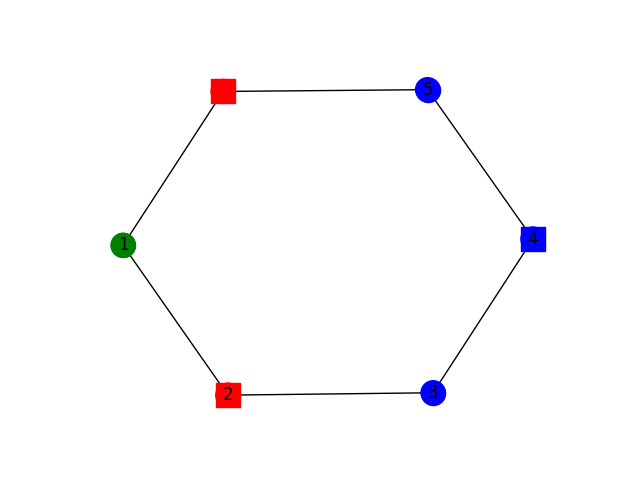
\includegraphics[scale=0.4]{./img/figures/ring_3_graph.png}\\
	\caption{Graph for [[3,1,$\frac{1}{2}$]] ring code}
        
	\label{fig: ring_graph}
	\end{center}
\end{figure}
